\documentclass[10pt]{article}

% amsmath package, useful for mathematical formulas
\usepackage{amsmath}
% amssymb package, useful for mathematical symbols
\usepackage{amssymb}

% graphicx package, useful for including eps and pdf graphics
% include graphics with the command \includegraphics
\usepackage{graphicx}

% cite package, to clean up citations in the main text. Do not remove.
\usepackage{cite}

\usepackage{color} 

% Use doublespacing - comment out for single spacing
\usepackage{setspace} 
\doublespacing

% Text layout
\topmargin 0.0cm
\oddsidemargin 0.5cm
\evensidemargin 0.5cm
\textwidth 16cm 
\textheight 21cm

% Bold the 'Figure #' in the caption and separate it with a period
% Captions will be left justified
\usepackage[labelfont=bf,labelsep=period,justification=raggedright]{caption}

% Use the PLoS provided bibtex style
\bibliographystyle{plos2009}

% Remove brackets from numbering in List of References
\makeatletter
\renewcommand{\@biblabel}[1]{\quad#1.}
\makeatother


% Leave date blank
\date{}

\pagestyle{myheadings}
%% ** EDIT HERE **


%% ** EDIT HERE **
%% PLEASE INCLUDE ALL MACROS BELOW

% figure files reside in the figures/ directory
\graphicspath{
{figures/}
}

%% END MACROS SECTION

\begin{document}

% Title must be 150 characters or less
\begin{flushleft}
{\Large
\textbf{Title}
}
% Insert Author names, affiliations and corresponding author email.
\\
Author1$^{1}$, 
Author2$^{2}$, 
Author3$^{3,\ast}$
\\
\bf{1} Author1 Dept/Program/Center, Institution Name, City, State, Country
\\
\bf{2} Author2 Dept/Program/Center, Institution Name, City, State, Country
\\
\bf{3} Author3 Dept/Program/Center, Institution Name, City, State, Country
\\
$\ast$ E-mail: Corresponding author@institute.edu
\end{flushleft}



% Please keep the abstract between 250 and 300 words
\section*{Abstract}



% Please keep the Author Summary between 150 and 200 words
% Use first person. PLoS ONE authors please skip this step. 
% Author Summary not valid for PLoS ONE submissions.   
\section*{Author Summary}



\section*{Introduction}

The adaptive immune response induced during an acute influenza A virus infection is a complex web of defense mechanisms able to control all but the most virulent strains.  Elegant studies in the mouse model have described in detail the induction phase of the adaptive response, including dendritic cell- delivery of antigen-specific cargos to the lymph node immunocytes \cite{Maines2008, Saenz2010, Hatta2010}, temporal and spatial details of precursor T and B cell activation within the lymph node architecture [Legge and Braciale 2006], and functional capabilities of resulting effector lymphocytes [La Gruta and Doherty 2006].  In contrast to the induction phase of the response, less is known about the temporal and spatial constraints on the effector phase of the response and how activated lymphocytes leaving regional lymph nodes efficiently ‘search’ for the infected tissue, often called the lymphocyte diaspora \cite{Marshall2001}. 

Mathematical models using mouse model data have simulated the evolution of the immune response and its impact on viral kinetics \cite{Handel2008, Lee2009, Miao2010, Handel2010, Wu2011}.  Such whole-response modeling has considerable potential in selecting the most promising strategies of vaccination and therapy, thus avoiding subsequent expensive animal and human trials.    Models using differential equations to predict temporal events, however, do not account for spatial characteristics of cell behavior, and must make assumptions about the efficiency of each functional component in the model. 

Here we focus on the time and physical constraints of the lymphocyte diaspora.  How do very small foci of infected tissue attract limited numbers of activated CD8 T cells, necessary for infection control \cite{Allan1990} [La Gruta and Doherty 2006], after release into the systemic vascular system which services non-infected tissue orders of magnitude larger than the target infected tissue?  A host of cytokines and chemokines secreted by infected cells are critical in directing immune cells to sites of infection \cite{Kawai1999, Sallusto2000, Zhao2000, Dufour2002, Thelen2008, Sigmundsdottir2008, Sallusto2008, Bromley2008, Kohlmeier2008}.  While each chemokine has been studied in detail for receptor specificity and function in knockout models, the details of chemokine local concentration, function and efficiency are difficult to examine in a virus-infected whole animal model.

Using an agent-based model (ABM) designed to test the spatial demands on the effector phase, we examined the homing of activated cytotoxic T lymphocytes (CTL) to infected foci in the lung and how chemokines secreted by infected epithelial cells contributed to infection control.   Our data on viral secretion and chemokine secretion patterns from human epithelial cells infected in vitro by three different influenza virus strains \cite{Mitchell2011}, combined with mouse model data on CTL production and the resolution of influenza infections reported in the literature, were used to construct the model. In our modeling environment we observed different efficiencies of control for the three influenza viruses dependent on chemokine kinetics and CTL search constraints.



% You may title this section "Methods" or "Models". 
% "Models" is not a valid title for PLoS ONE authors. However, PLoS ONE
% authors may use "Analysis" 
\section*{Models}


\subsection*{Computational Modeling}

\begin{figure}[ht!]
\begin{center}
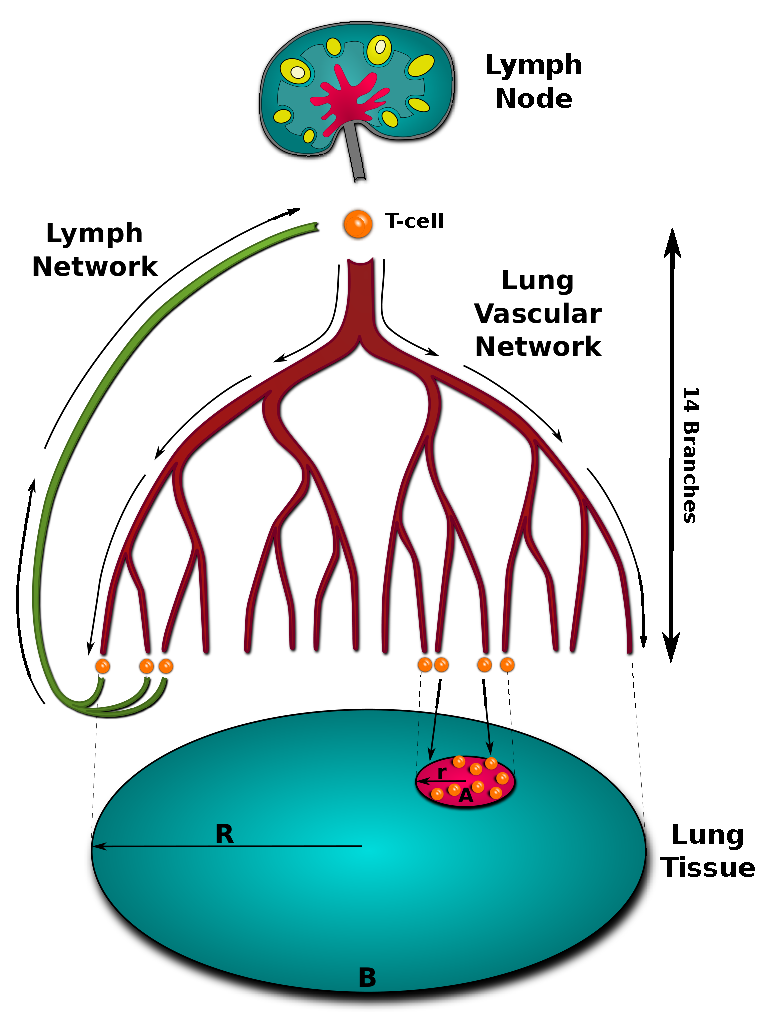
\includegraphics[width=0.4\textwidth]{SystemChart}
\end{center}
\caption{A region of infected tissue of radius $r$ (shaded region $A$) expressing chemokines and inflammatory signals. This region is surrounded by region $B$ which does not have any infected cells and hence does not express either chemokines or inflammatory signals. The $2^{14}$ capillaries (red circles) are distributed evenly throughout the entire lung (region $A$ and $B$).}
\label{fig:systemchart}
\end{figure}

% FIXME: The main goal of this paper is to compare chemokine signaling effectiveness between infections from different strains of influenza. Our study looks at separate infections from three different strains: seasonal, avian, and swine. Futhermore, we compare the roles of two established signaling molecules: CXCL10 (IP-10) and CCL5 (RANTES).

FIXME: Need to say somewhere that we simulate a generic chemokinetic signal that abstracts X, Y, and Z.

Computational modeling was conducted using Cycells [REF], a modeling platform for implementing two- or three-dimensional agent-based simulations of immune response [REF]. A simplified model of T-Cell activation and recirculation was implemented in Cycells (Fig 1) and simulations were conducted to measure efficiency of infection clearance under different environmental conditions. To model a growing infection, the lung was represented as a two dimensional sheet of healthy epithelial cells. Vasculature was represented as a binary tree with fourteen branches originating at a single lymph node. Activated T-cells descend through the vascular tree until chemotactic signal is detected, at which point they exit the vasculature and follow the [FIXME chemotactic/inflammatory] gradient to the site of infection. T-cells that do not encounter chemokine recirculate to the lymph node. Once at the site of infection, a T-Cell may encounter an infected epithelial cell and induce apoptosis.

The simulation begins when a single cell in the center of the tissue is infected. After the eclipse phase (incubation), the infected cell begins secreting virus and chemokine. Virus diffuses locally, infecting nearby cells, and continuing the cycle. The chemokine diffuses from secreting cells, thus increasing the size of the signaling area. After a delay, to simulate lymph node stimulation and T-Cell proliferation, activated T-cells begin exiting the lymph node and circulating through the vasculature to the tissue. Because T-Cells cannot choose their path through the branching network, we assume they arrive in tissue at random locations. Figure \ref{fig:modelchart} illustrates the model components 
(epithelial cells, T-cells, and particles) and how they transition between different states.


\subsection*{Model Definition}

\begin{figure}[ht!]
\begin{center}
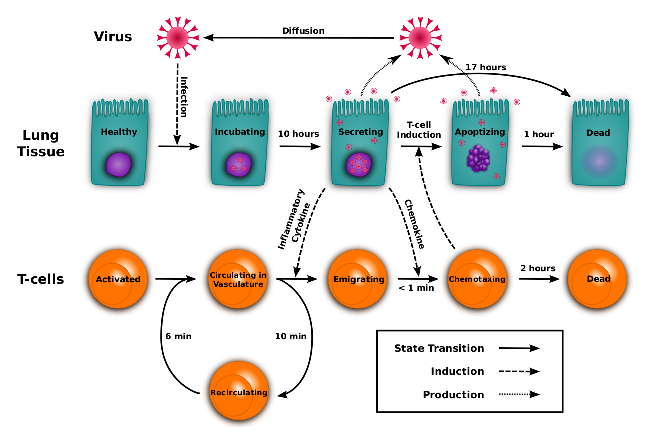
\includegraphics[width=\textwidth]{ModelChart}
\end{center}
\caption{Computational model: Components and state transitions.}
\label{fig:modelchart}
\end{figure}

Epithelial cells are stationary and can be in of five different states: \emph{healthy}, \emph{virus-incubating}, \emph{virus-expressing}, \emph{apoptotic}, and \emph{dead}. \emph{healthy} cells remain unchanged unless infected by virus. Once infected, there is a 10h incubation window before the cell transitions from {incubating} to \emph{expressing}. \emph{Expressing} cells secrete virus and chemokine for 17 hours and then die. \emph{Expressing} cells become \emph{apoptotic} if they encounter activated T-cells. Apoptoic cells continue to secrete virus and die one hour after their transition. \emph{Dead} cells remain inert and do not regenerate over the course of an infection.

T-cells have three states: \emph{searching}, \emph{recirculating}, and \emph{activated}. T-Cells begin emerging from the lymph node at five days post infection at the rate of 777 T-cells per hour for the duration of the simulation. T-Cells enter the vascular system in the \emph{searching} state, arriving at a random location on the lung's surface. \emph{searching} cells perform a random walk in the tissue for 10 minutes, after which they transition to \emph{circulating} if they fail to encounter chemokine. \emph{Circulating} cells spend six minutes recirculating to the lymph node where they are converted to \emph{searching} and reintroduced to a new random location in the lung. If a \emph{searching} T-Cell encounters chemokine, it immedaiately converts to \emph{activated} and begins climbing the chemotactic gradient to the source of infection. \emph{Activated} T-Cells move continuously up the gradient and if they encounter \emph{expressing} epithelial cells, the epithelial cell transitions \emph{apotosis}. Activated T-cells are removed from the simulation using an exponential decay rate with an average lifespan of two hours. 

The model contains two kinds of particles: virus and chemokine. Both are produced at constant rates by \emph{expressing} epithelial cells.  Virus diffuses through the lung tissue, infecting healthy cells probabilistically according to the local virus concentration. Chemokine diffuses across the tissue but has no
direct effect beyond activating T-Cells. Both particle types decay over time.


\subsection*{Parameters}

Define CyCells environment.  Talk about the need for spatial model.  Human/mouse scaling.  Parameter definitions. 

\begin{table}
\begin{tabular}{ | c | c | c | }
  \hline                        
  Paramter & Value & Source \\
  \hline
  Viral Diffusion & .0318 & Stokes-Einstein / Beau \\
  Viral Decay &  1/day & Soumya \\
  Chemokine Diffusion & .318 & Stokes-Einstein \\
  Chemokine Decay &  3.8508e-4/s & 30m half-life \\
  Infection Sensitivity &  2h/virion & [1] \\
  Incubation Time &  10h & Mitchell \\
  Expression Time &  16.7h & Mitchell \\
  Apoptosis Time & 1h & Fred \\
  T-Cell Production Rate & 777/h & Soumya, Miao fits \\ 
  Circulation Time & 6m & Fred, mouse model \\
  Search Time & 10m & Fred, mouse model \\
  T-Cell Speed (Search) & $30 \mu m/s$ & Fred ? \\
  T-Cell Speed (Activated) & $3 \mu m/s$ & Fred ?\\
  T-Cell Sensitivity & $100 ng/ml$ & See Results \\
  T-Cell Expected Kill Rate & 10m & Fred/Drew \\
  Cell Radius & $25 \mu m$ & Fred \\
  T-Cell Age (Active) & 2h & Fred \\
  T-Cell Age (Other) & 3d & Fred \\
  T-Cell Ramp Up Time & 5d & Icaris \\
  IgM Strength & Viral decay of 3/day after day 3 & Soumya [3] \\
  \hline  
\end{tabular}
\caption{Generic model parameters}
\label{table:parameters}
\end{table}


\begin{table}
\begin{center}
\begin{tabular}{ | r | c | c | }
  \hline                        
  Paramter & Value & Source \\
  \hline
  IP-10 Production Rate &  & [2]\\
  Avian H5N1 & 7.2e-5 ng/s$\cdot$cell & \\
  Seasonal H1N1 & 9.3e-5 ng/s$\cdot$cell& \\
  Pandemic H1N1 & 6.3e-5 ng/s$\cdot$cell& \\
  \hline
  RANTES Production Rate & & [2] \\
  Avian H5N1 & 3.9e-5 ng/s$\cdot$cell& \\
  Seasonal H1N1 & 1.3e-6 ng/s$\cdot$cell& \\
  Pandemic H1N1 & 1.4e-6 ng/s$\cdot$cell& \\
  \hline
  Virus Production Rate &  & Mitchell \\
  Avian H5N1 & 5.4e-5 PFU/s$\cdot$cell& \\
  Seasonal H1N1 & 3.8e-4 PFU/s$\cdot$cell& \\
  Pandemic H1N1 & 5.1e-3 PFU/s$\cdot$cell& \\  
  \hline  
\end{tabular}
\caption{Strain specific model parameters}
\label{table:strains}
\end{center}
\end{table}

\begin{itemize}
\item[1] The molecular concentration where there is one molecule per eptithelial cell volume is 1.53e-17 mol/ml.  Thus, if you multiply the local viral concentration by 9.05e12 you get an infection event after two hours given that concentration.  This probability scales linearly with the viral concentration.
\item[2] These are calculated off of Fred's new data sets using the Mitchell ODE model and parameters as a basis.
\item[3] IgM is represented by increasing the viral decay rate to 3/day after the third day of the simulation.
\end{itemize}


% Results and Discussion can be combined.
\section*{Results}

\subsection*{Chemokine production}

Chemokine data were collected from epithelial monolayers infected with influenza strains, as described in \cite{Mitchell2011} (Fig.~\ref{fig:data}).  IP-10 concentration increases were observed by 8h p.i., and RANTES by 16h p.i..  To estimate per-cell production rates, we extended the ODE model of Ref. \cite{Mitchell2011} to represent chemokine production from infected cells.  Model fits were generated for three influenza strains (Fig.~\ref{fig:data}) using a genetic algorithm [REF: GA-ref].  The model estimates are shown in Table~\ref{table:strains}.  These chemokine expression rates are consistent for each chemokine across the different strains except that the RANTES rate is higher in avian H5N1.  There is no discernible correlation between viral production and induced chemokine production across the three strains of influenza.

\begin{figure}[ht!]
\begin{center}
 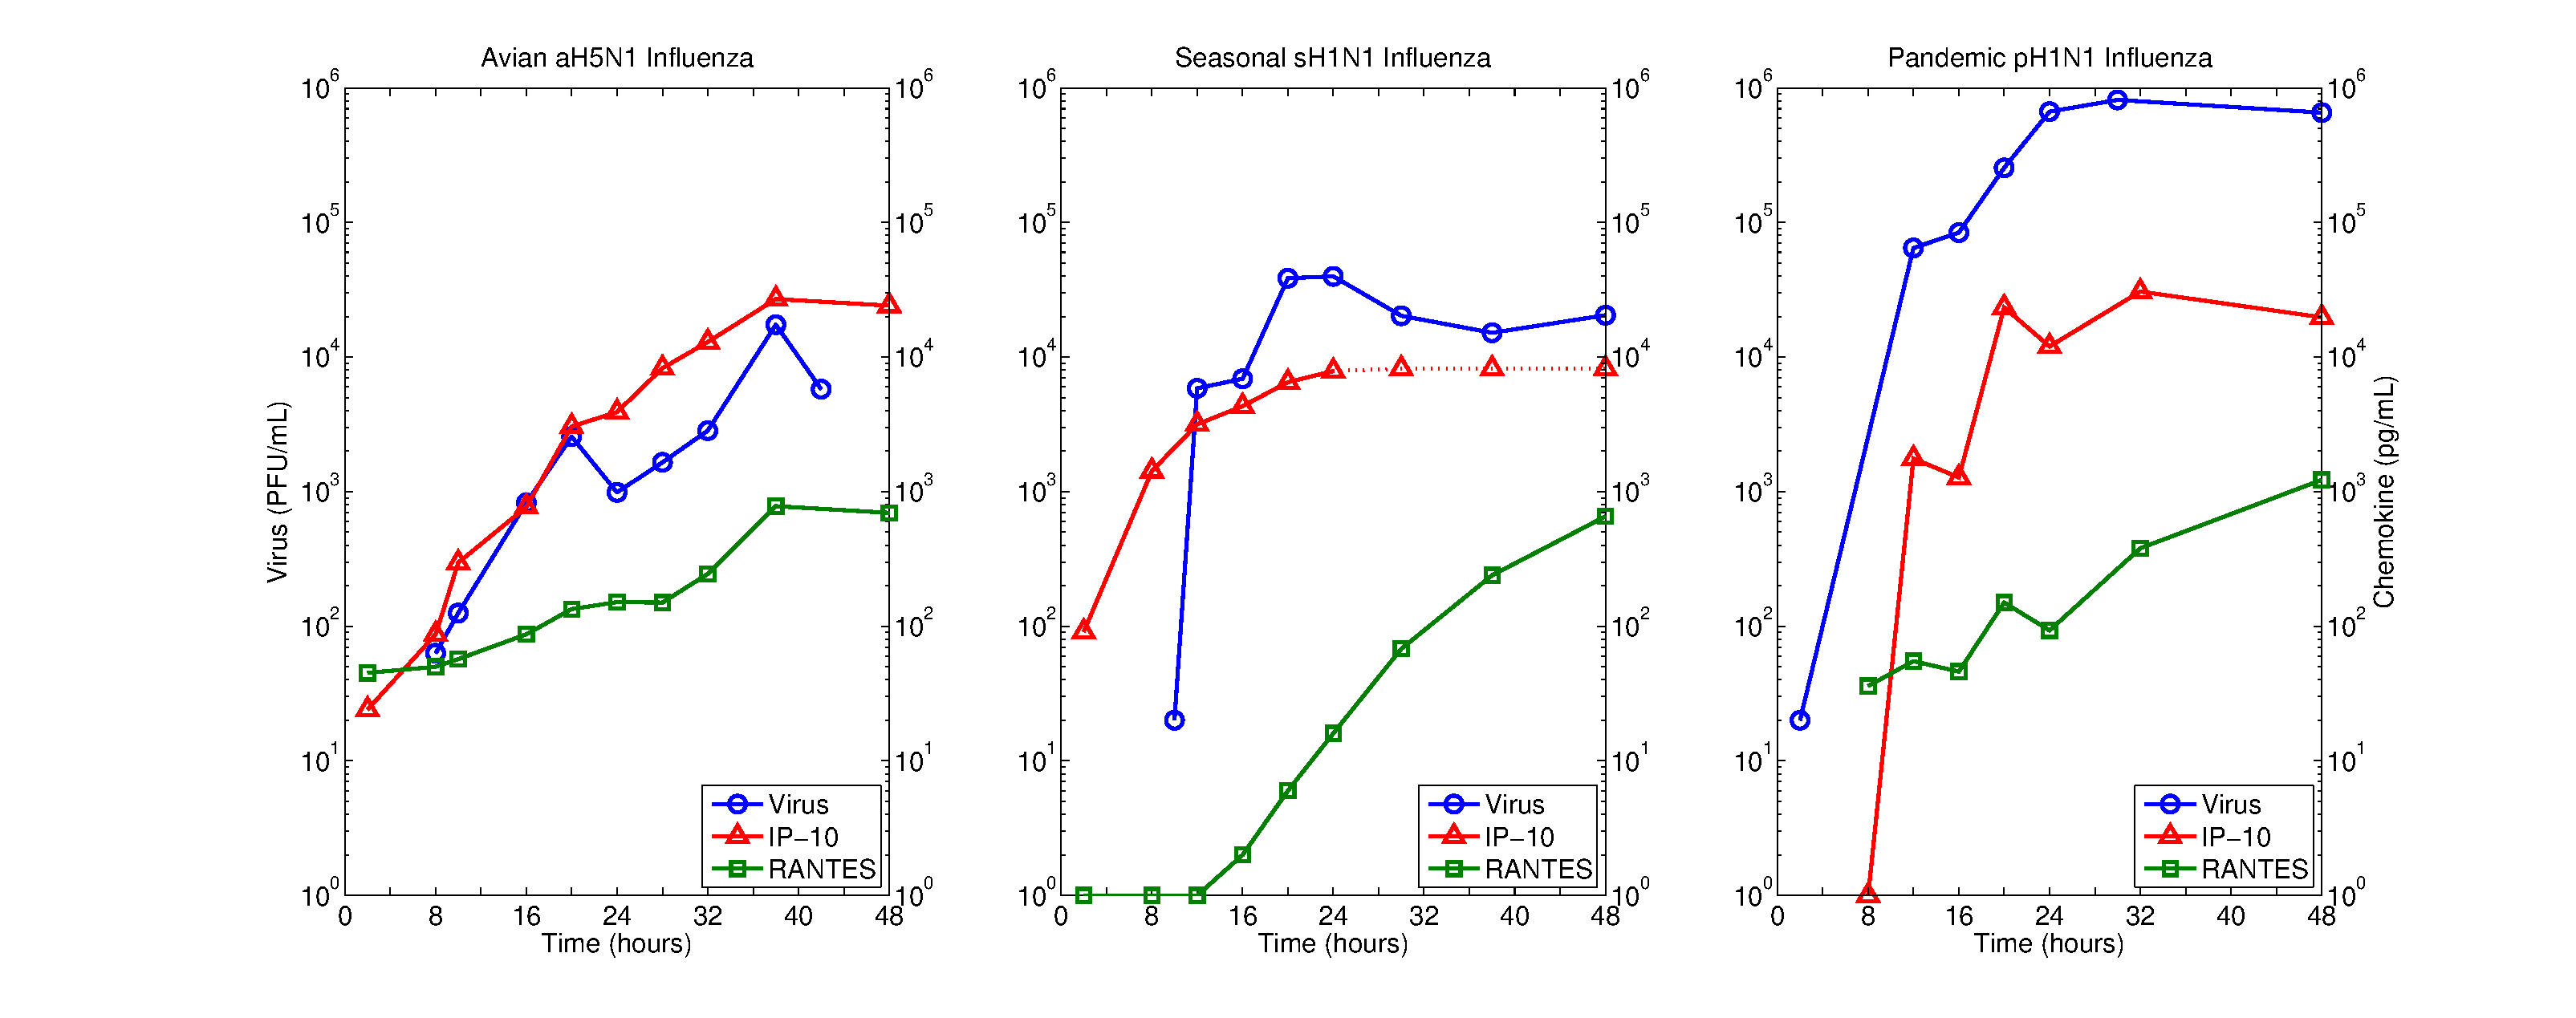
\includegraphics[width=\textwidth]{data}
 \end{center}
\caption{Empirical data of viral and cytokine titer for three strains of influenza: Avian H5N1 (A), Seasonal sH1N1 (B), and Pandemic pH1N1 (C).  For each strain, the viral load (blue circle) is shown in PFU/ml and the chemokines IP-10 (red triangle) and RANTES (green square) are shown in ng/ml.} 
 \label{fig:data}
\end{figure}

\subsection*{Stochastic modeling effects}

% [FIXME-DREW: Shouldn't we do 30 runs instead of 10 to get statistical significance?   Drew: Sure, I can always do more runs, I did 10 just to have a figure to look at.]

Unlike ODE models, which are deterministic, stochastic models such as CyCells can produce different results on different runs (Figure~\ref{fig:variance}).  To test the strength of this effect, we ran each model ten (MORE?) times using the default parameters given in Table~\ref{table:parameters}, finding that the variance of infected cells was X.  Each run took as input the calculated viral production and chemokine production rates for the three different strains of influenza, reporting as output the total number of infected cells, including incubating, virus secreting and apoptotic, but not including dead cells.  The figures thus approximate plaque growth over time.

Overlaying multiple runs on a single plot reveals a slight growth rate transition 3 days p.i., which reflects the presence of IgM.  In addition, for each infection the number of infected cells declines quickly at day five due to the T-cell response. 

The three strains show different levels of virulence, consistent with the results found in Mitchell (Fig.~\ref{fig:variance}).  The rapid growth of the pandemic H1N1 prevents the immune response from containing the infection.  By the time T-Cells arrive, the plaque is too large for them  to cover effectively.  Because pH1N1 is produced so quickly, the window of opportunity for T-Cells to gain ground is too small (Discussion).  aH5N1 is cleared completely, sH1N1 is contained but not fully cleared, and pH5N1 recovers and continues to expand.

\begin{figure}[ht!]
\begin{center}
 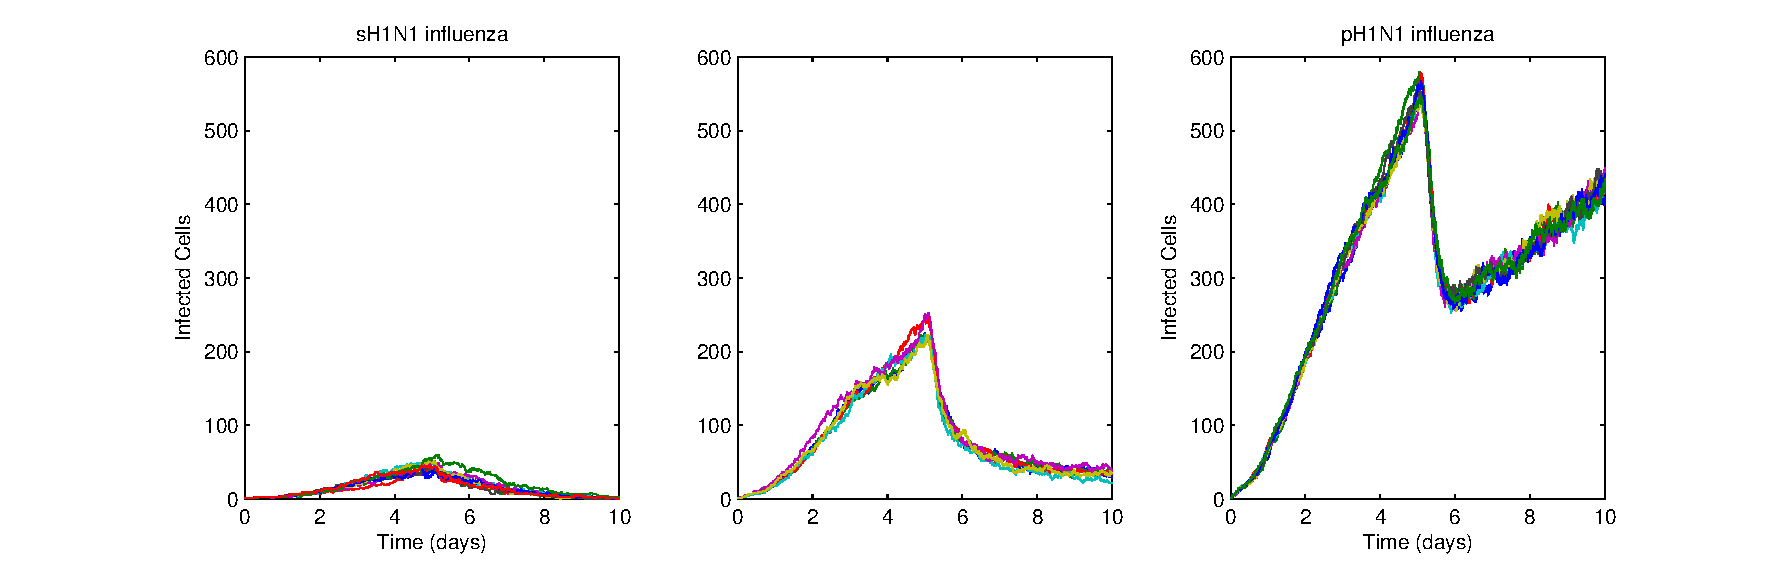
\includegraphics[width=\textwidth]{variance}
 \end{center}
\caption{Model results: Time series plots of ten runs of aH5N1 (A), sH1N1 (B), and pH1N1 (C) infections. IP-10 and RANTES were simulated in each run, except for aH5N1, which  produced only RANTES.  The ten runs were initialized identically for each strain.  Each simulation was run with identical T-cell sensitivity to chemokine (100 ng/ml).} 
 \label{fig:variance}
\end{figure}


\subsection*{T-cell sensitivity to chemokine}

T-Cells exit a capillary when they sense inflammatory cytokine and then follow a second signal, the chemokine gradient.  We use the chemokine gradient as a proxy for the inflammatory signal.  Figure \ref{fig:cycells} shows chemokine concentrated around virus secreting cells.  T-cell sensitivity determines how much aggregate chemokine signal is required to detect the gradient.

To test for the minimum concentration of cytokine/chemokine signal required to recruit T-Cells from capillary, we simulated sensitivity levels ranging over seven orders of magnitude. We find a threshold (Fig.~\ref{fig:sensitivity}) between the concentrations of (FIXME: new values) 1e-18 and 1e-19 (1e-19 and 1e-20 for pH1N1), above which there is no discernible effect on infection kinetics.  Because multiple T-cells in the same area do not increase the rate at which  apoptosis is induced, we hypothesize that a critical number of T-cells is required to clear an infection, above which there is no additional benefit from increasing numbers.  For consistency, we standardized all subsequent model runs to  sensitivity of 1e-22.

\begin{figure}[ht!]
\begin{center}
 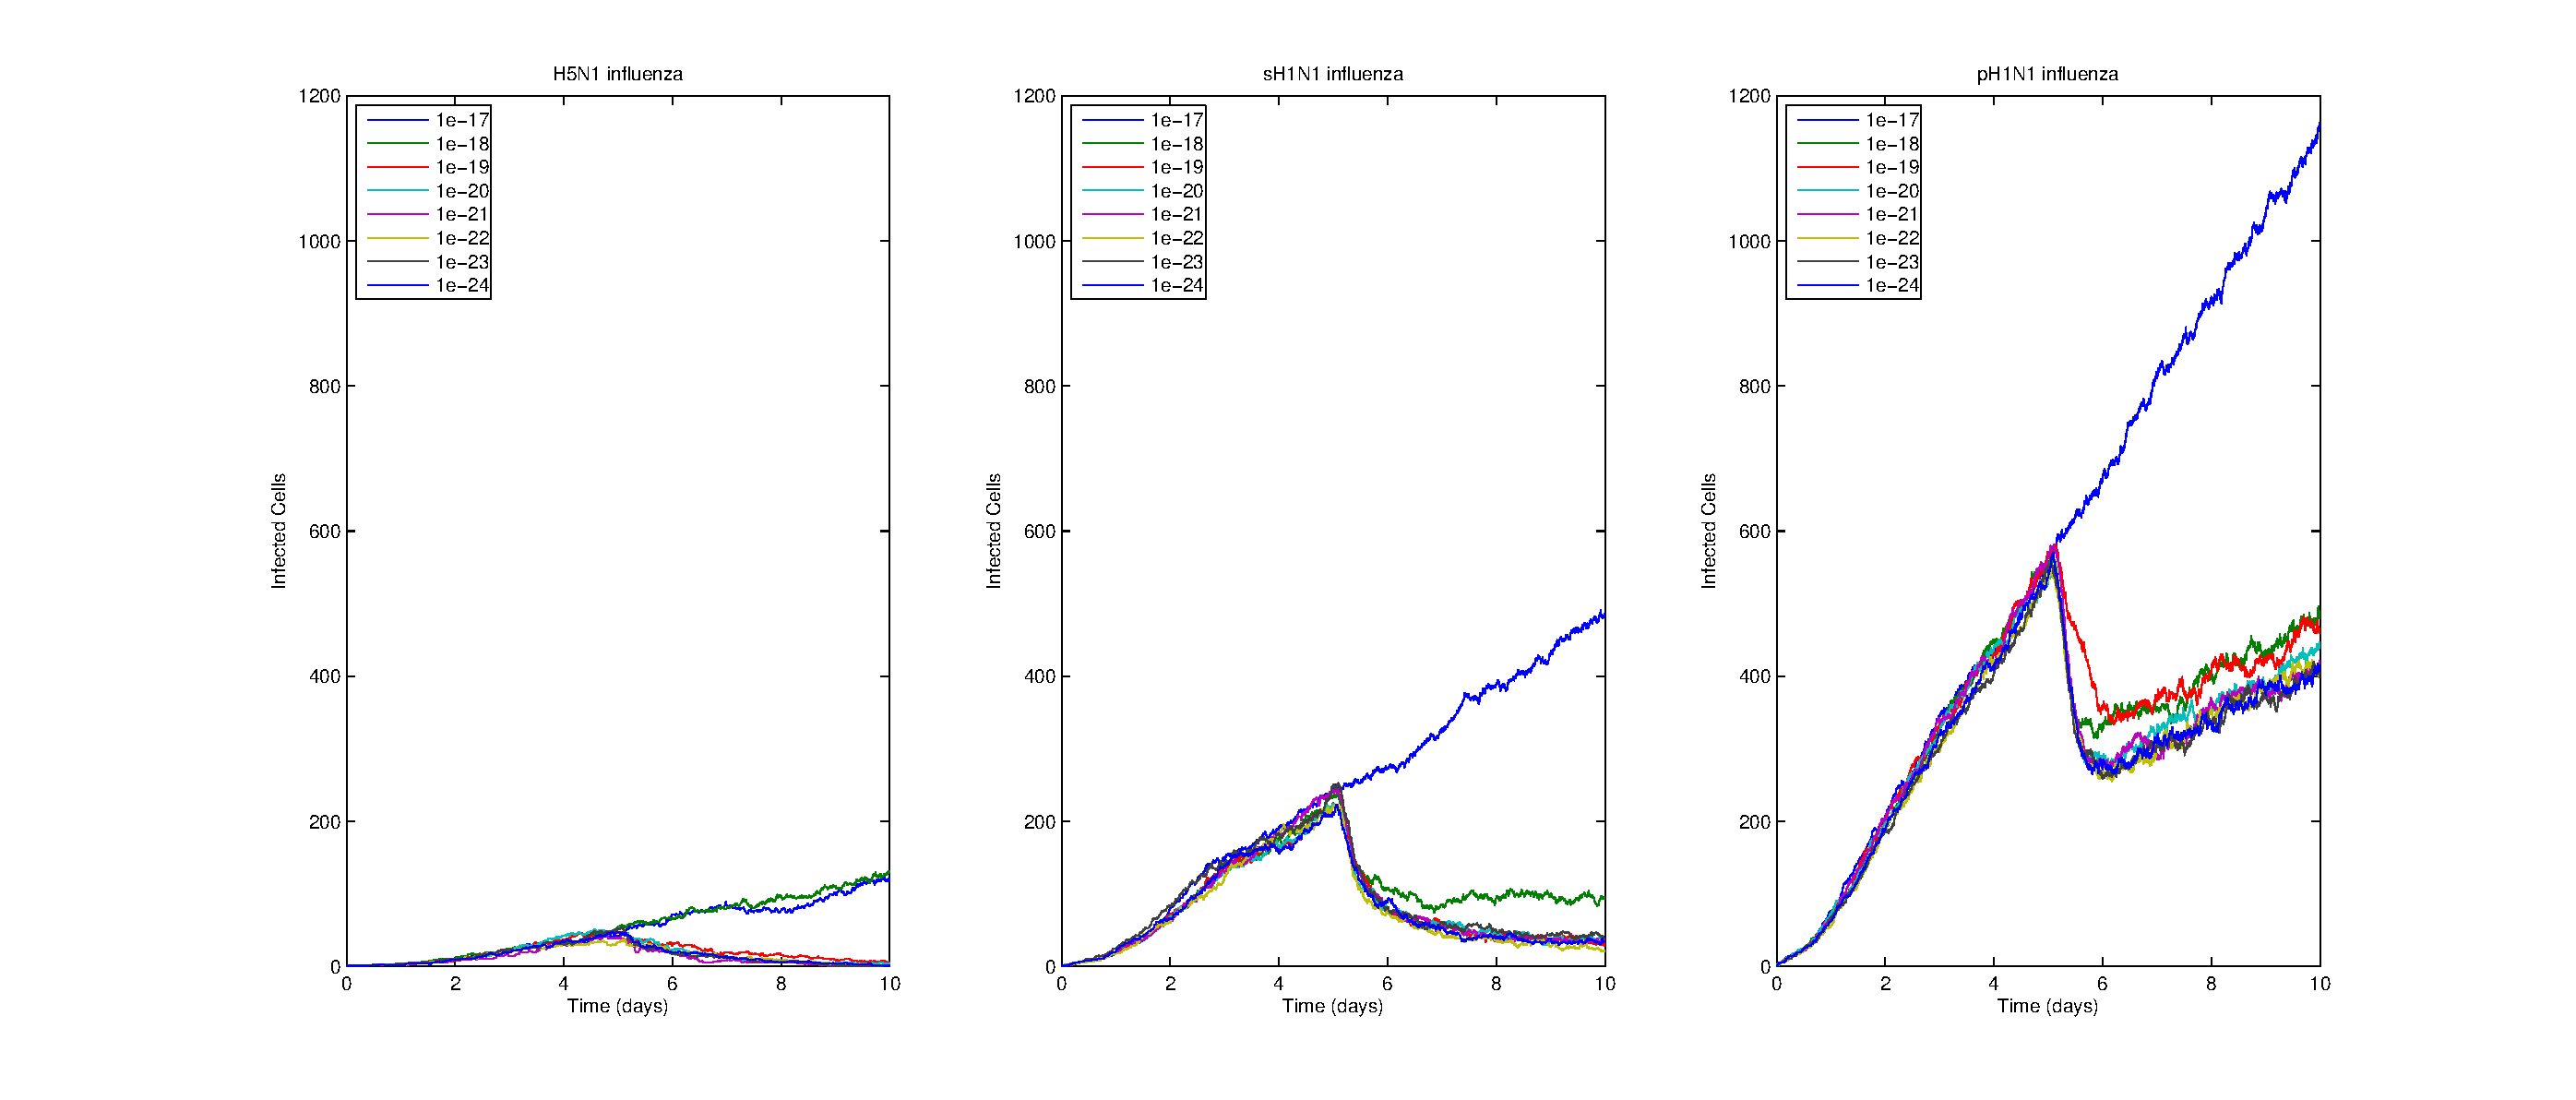
\includegraphics[width=\textwidth]{sensitivity}
 \end{center}
\caption{Varying T-cell sensitivity to chemokine in the model: H5N1 model results use RANTES  only, and sH1N1 and pH1N1 use both IP-10 and RANTES. Total number of infected, expressing and apoptotic cells are plotted for each infection.  The sensitivity value specifies the minimum level of chemokine concentration required for T-cells to detect it. } 
 \label{fig:sensitivity}
\end{figure}


\subsection*{Chemokine combinations}

Because aH5N1 has been shown to surpress the production of interferon \cite{Mitchell2011} we hypothesize that it renders IP-10 is ineffectual (FIXME: need to clean this up).  This may explain why aH5N1 has a much higher secretion rate for RANTES than the other two strains (Table~\ref{table:strains}).  Because of this behavior, IP-10 was not included in the aH5N1 models.

Four models runs were performed for each strain (two for aH5N1) to look at how the presence and/or lack of specific chemokines affect the efficacy of the simulated immune response (Fig.~\ref{fig:chemokine}).  The lack of both chemokines leads to runaway infections in all three strains.  The presence of only RANTES is enough to contain the aH5N1 infection, but is weaker than IP-10 in both H1N1 strains.  IP-10 alone proves to be just as effective and both IP-10 and RANTES, suggesting that RANTES does not play a significant role in infections that stimulate an IP-10 response.

\begin{figure}[ht!]
\begin{center}
	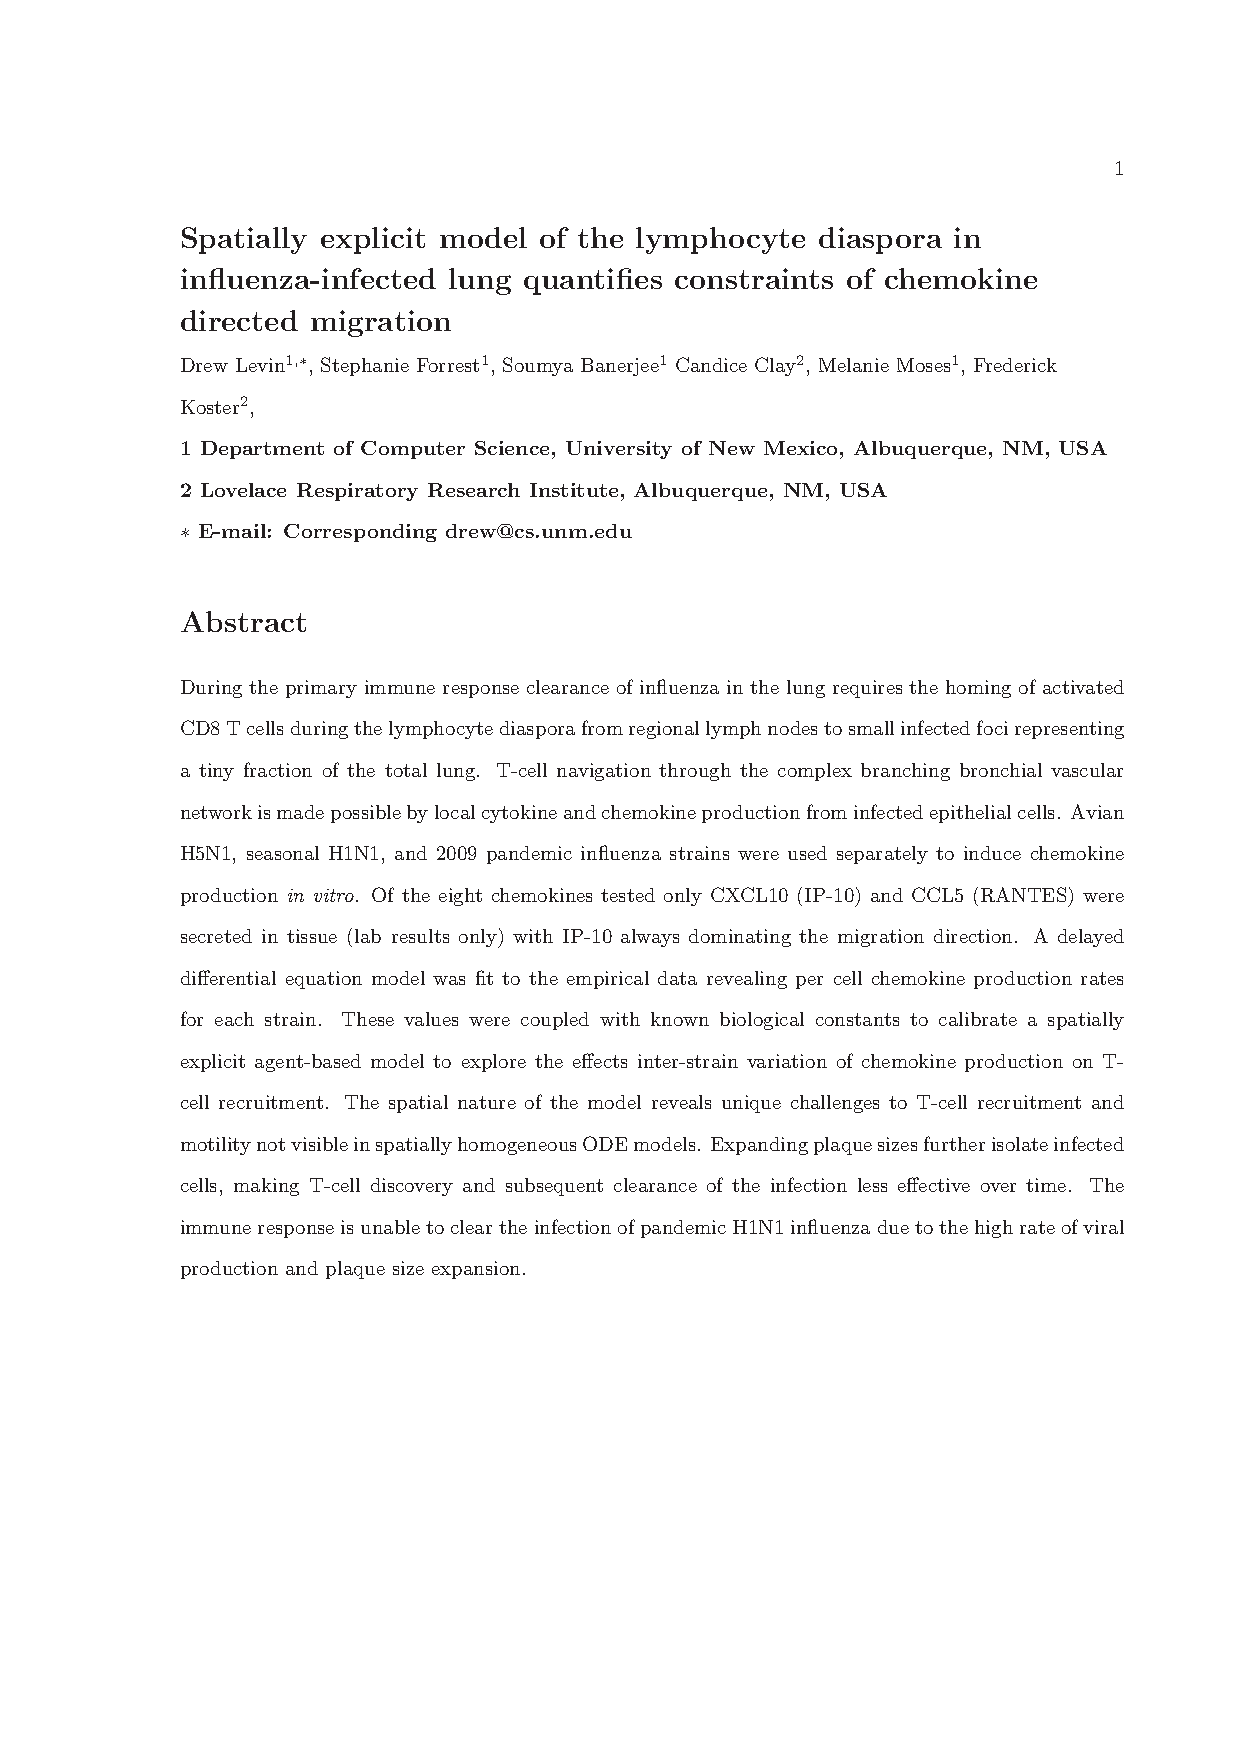
\includegraphics[width=\textwidth]{chemokine}
	\caption{Effects of different chemokine combinations.  A) aH5N1 does not stimulate an IP-10 response.  B-C) sH1N1 and pH1N1 show no significant difference between IP-10 alone versus IP-10 and RANTES combined.}
	\label{fig:chemokine}
\end{center}
\end{figure}



\subsection*{Spatial effects}

Spatial effects of viral and chemokine diffusion play an important role in both the spread and clearance of infection.  Free virus particles diffuse from virus secreting cells and infect healthy cells.  Chemokine produced by infected cells attracts T-cells to the infected cells.  Although virus is produced at a higher rate than chemokine, it diffuses much more slowly because it is a larger particle.  Chemokine diffusion, however, is limited by higher decay rates than the virus.  These countervaling effects result in similar spatial profiles for the two particle types (Fig.~\ref{fig:cycells}).

Early in the infection (up to day 4) the plaque is dominated by active (incubating and secreting) cells, and dead cells are rare. Over time, cells in the plaque's interior die, so active cells comprise a decreasing proportion of the total. T-cells arrive at day 5 and begin to killing the plentiful virus-expressing cells. By day 6 many of the expressing cells have been eliminated and the plaque is dominated by dead cells.  In the H5N1 example, the plaque is dense, so the secreting cells can be found easily and the infection is eliminated.  In both H1N1 simulations, however, secreting cells are not eliminated.  In these cases, expressing cells account for at most 10\% of the active cell population and less than  1\% of the total plaque at 6 days p.i.  T-cells still accumulate, but they arrive at a slower rate than the plaque's rate of growth. This leads to a lower probability of T-cells finding and killing the remaining expressing cells, and the infection is able to recover and resume growth.   The regions of concentrated chemokine trail the cell and virus spatial layout.  It takes time for newly secreting cells to produce chemokine and for old pockets of chemokine to decay away.  Thus, T-cells, which rely on the chemokine gradient to find infected cells, often lag behind changes in the plaque.  The delayed response and the low proportion of virus secreting cells prevent T-cells from clearing the infection completely.

\begin{figure}[ht!]
\begin{center}
 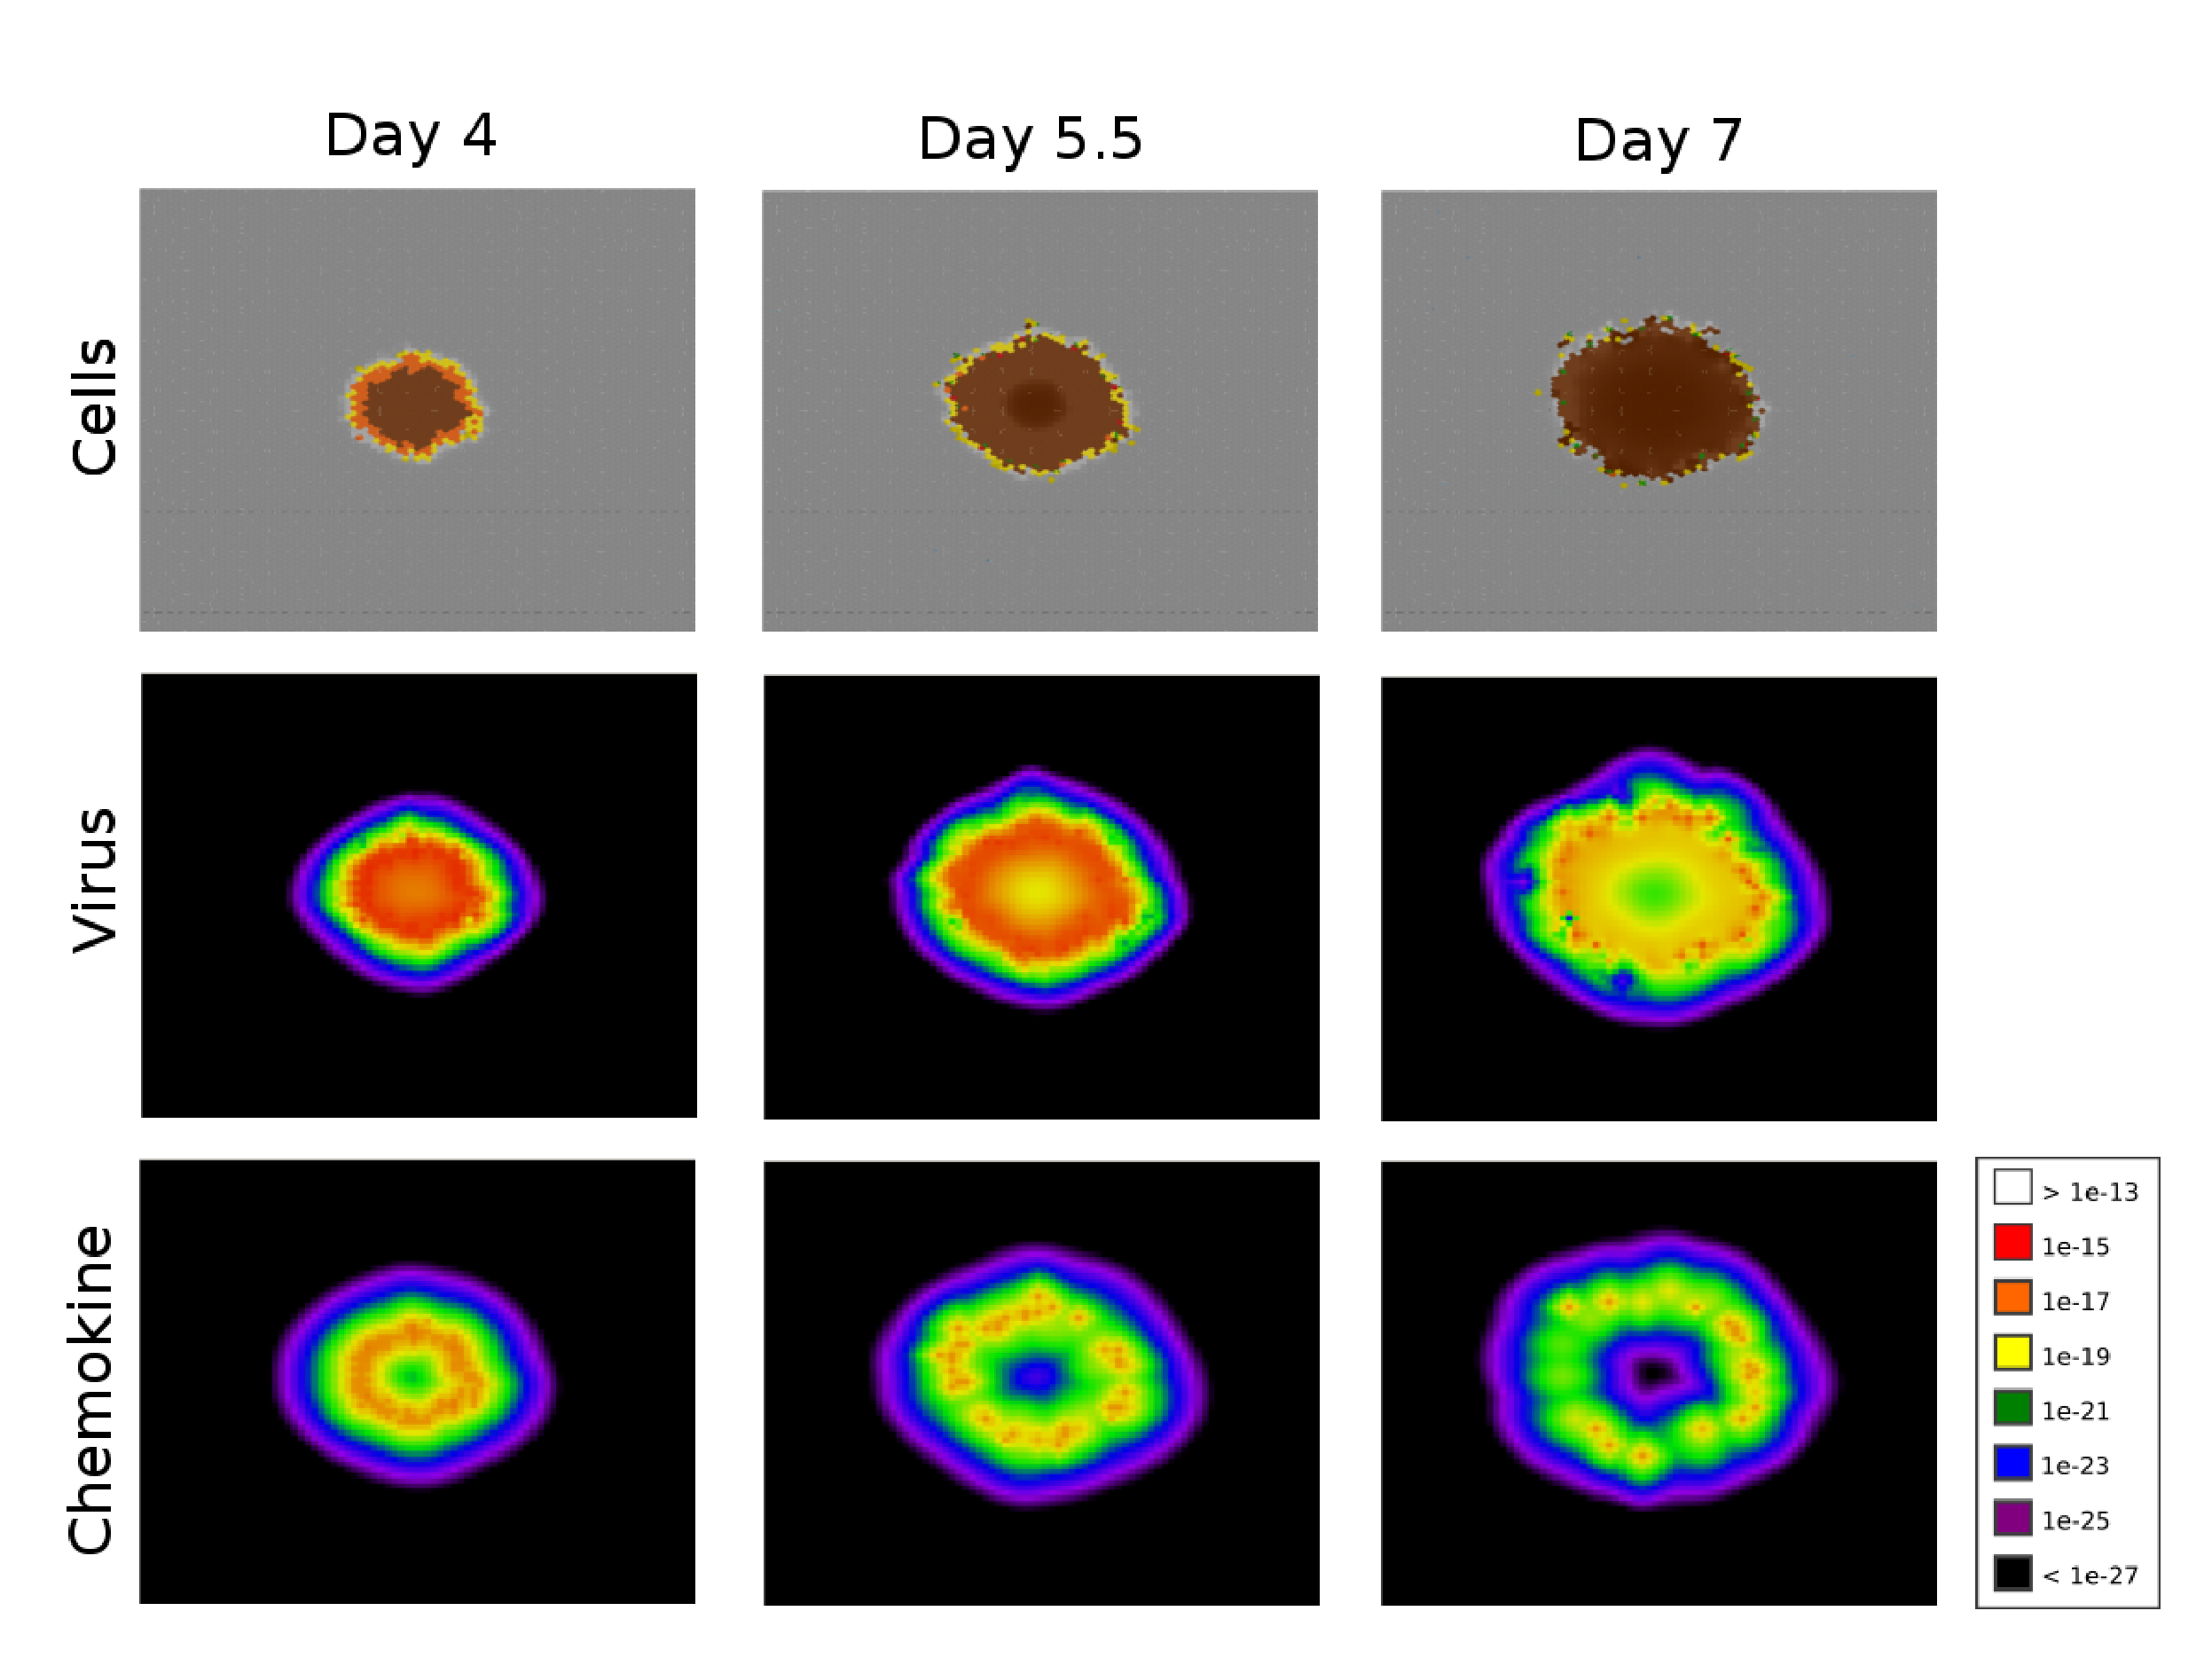
\includegraphics[width=\textwidth]{cycells}
 \end{center}
\caption{Example simulated sH1N1 infection. Screenshots taken at Day 4, Day 5.5, and Day 7.  The top row shows the spreading focus of infection  through the color coding of individual cells:  healthy cells in uninfected tissue (gray),  virus-incubating cells (yellow), virus-secreting cells (orange), apoptotic cells (red), dead cells (brown), and T-cells introduced at day 5 (green).  Free virus and chemokine particles are represented by compartmentalized concentrations of mols/ml and ng/ml (see the legend in the bottom right).} 
 \label{fig:cycells}
\end{figure}




\subsection*{Infection rebound}

%FIXME-DREW-FRED: expressing, actively presenting viral peptides, secreting, viral-secreting, etc.  Pls. choose one of these terms, introduce its synomys early, and then be consistent for the rest of the paper. Drew: Healthy, Virus-Incubating or Incubating, Virus-Secreting or Secreting, Apoptotic, Dead.

The immune response fails to clear sH1N1 completely and is unable to contain the pH1N1 (Fig. \ref{fig:variance}).  This appears to be an artifact of the spatial nature of the ABM.  Why can the immune response create an immediate decrease in the number of pH1N1 infected cells at day 5, only to fail in the same endeavor two days later?   Figure \ref{fig:variance} reports only the number of infected cells, not counting dead cells in the focus of infection (FOI).  Further, T-Cells induce apoptosis in virus-secreting cells, but not in virus-incubating cells.  At day 5.5, the ratio of secreting cells to the total FOI is high (Fig.~\ref{fig:cycells}). By day 7, the ratio of plaque size to the number of secreting cells is approximately 100:1 for both the pH1N1 and sH1N1 strains.  However the greater replication rate of pH1N1 widens the gap (Fig.~\ref{fig:plaquesize}C) whereas the lower replication rate of sH1N1 allows the T-cells to keep up, even after day seven, leading to control (but not elimination) of the sH1N1 infection.

A cell infected with pH1N1 produces new virus at the rate of 5.08e-3 PFU/s [FIXME: Where does this come from? IS this our data, model results, or what? Drew: from Mitchell et al].  That is, a new viral particle is produced approximately every 200 seconds.  Assuming that virus particle secretion continues for one hour after apoptosis is initiated, the best a T-Cell can do is to limit a single infected cell to producing 18 new viral particles.  Without additional immune responses, T-Cells alone cannot contain the pH1N1 infection.  In contrast, the sH1N1 virus-secreting cell produces a new virus particle every 2,643 seconds, so the T-cell can limit a single infected cell to producing 1.3 viral particles in the one-hour window.  Avian H5N1 virus-secreting cells produce only 0.2 viral particles in the interval after T-cell detection. 


\begin{figure}[ht!]
\begin{center}
 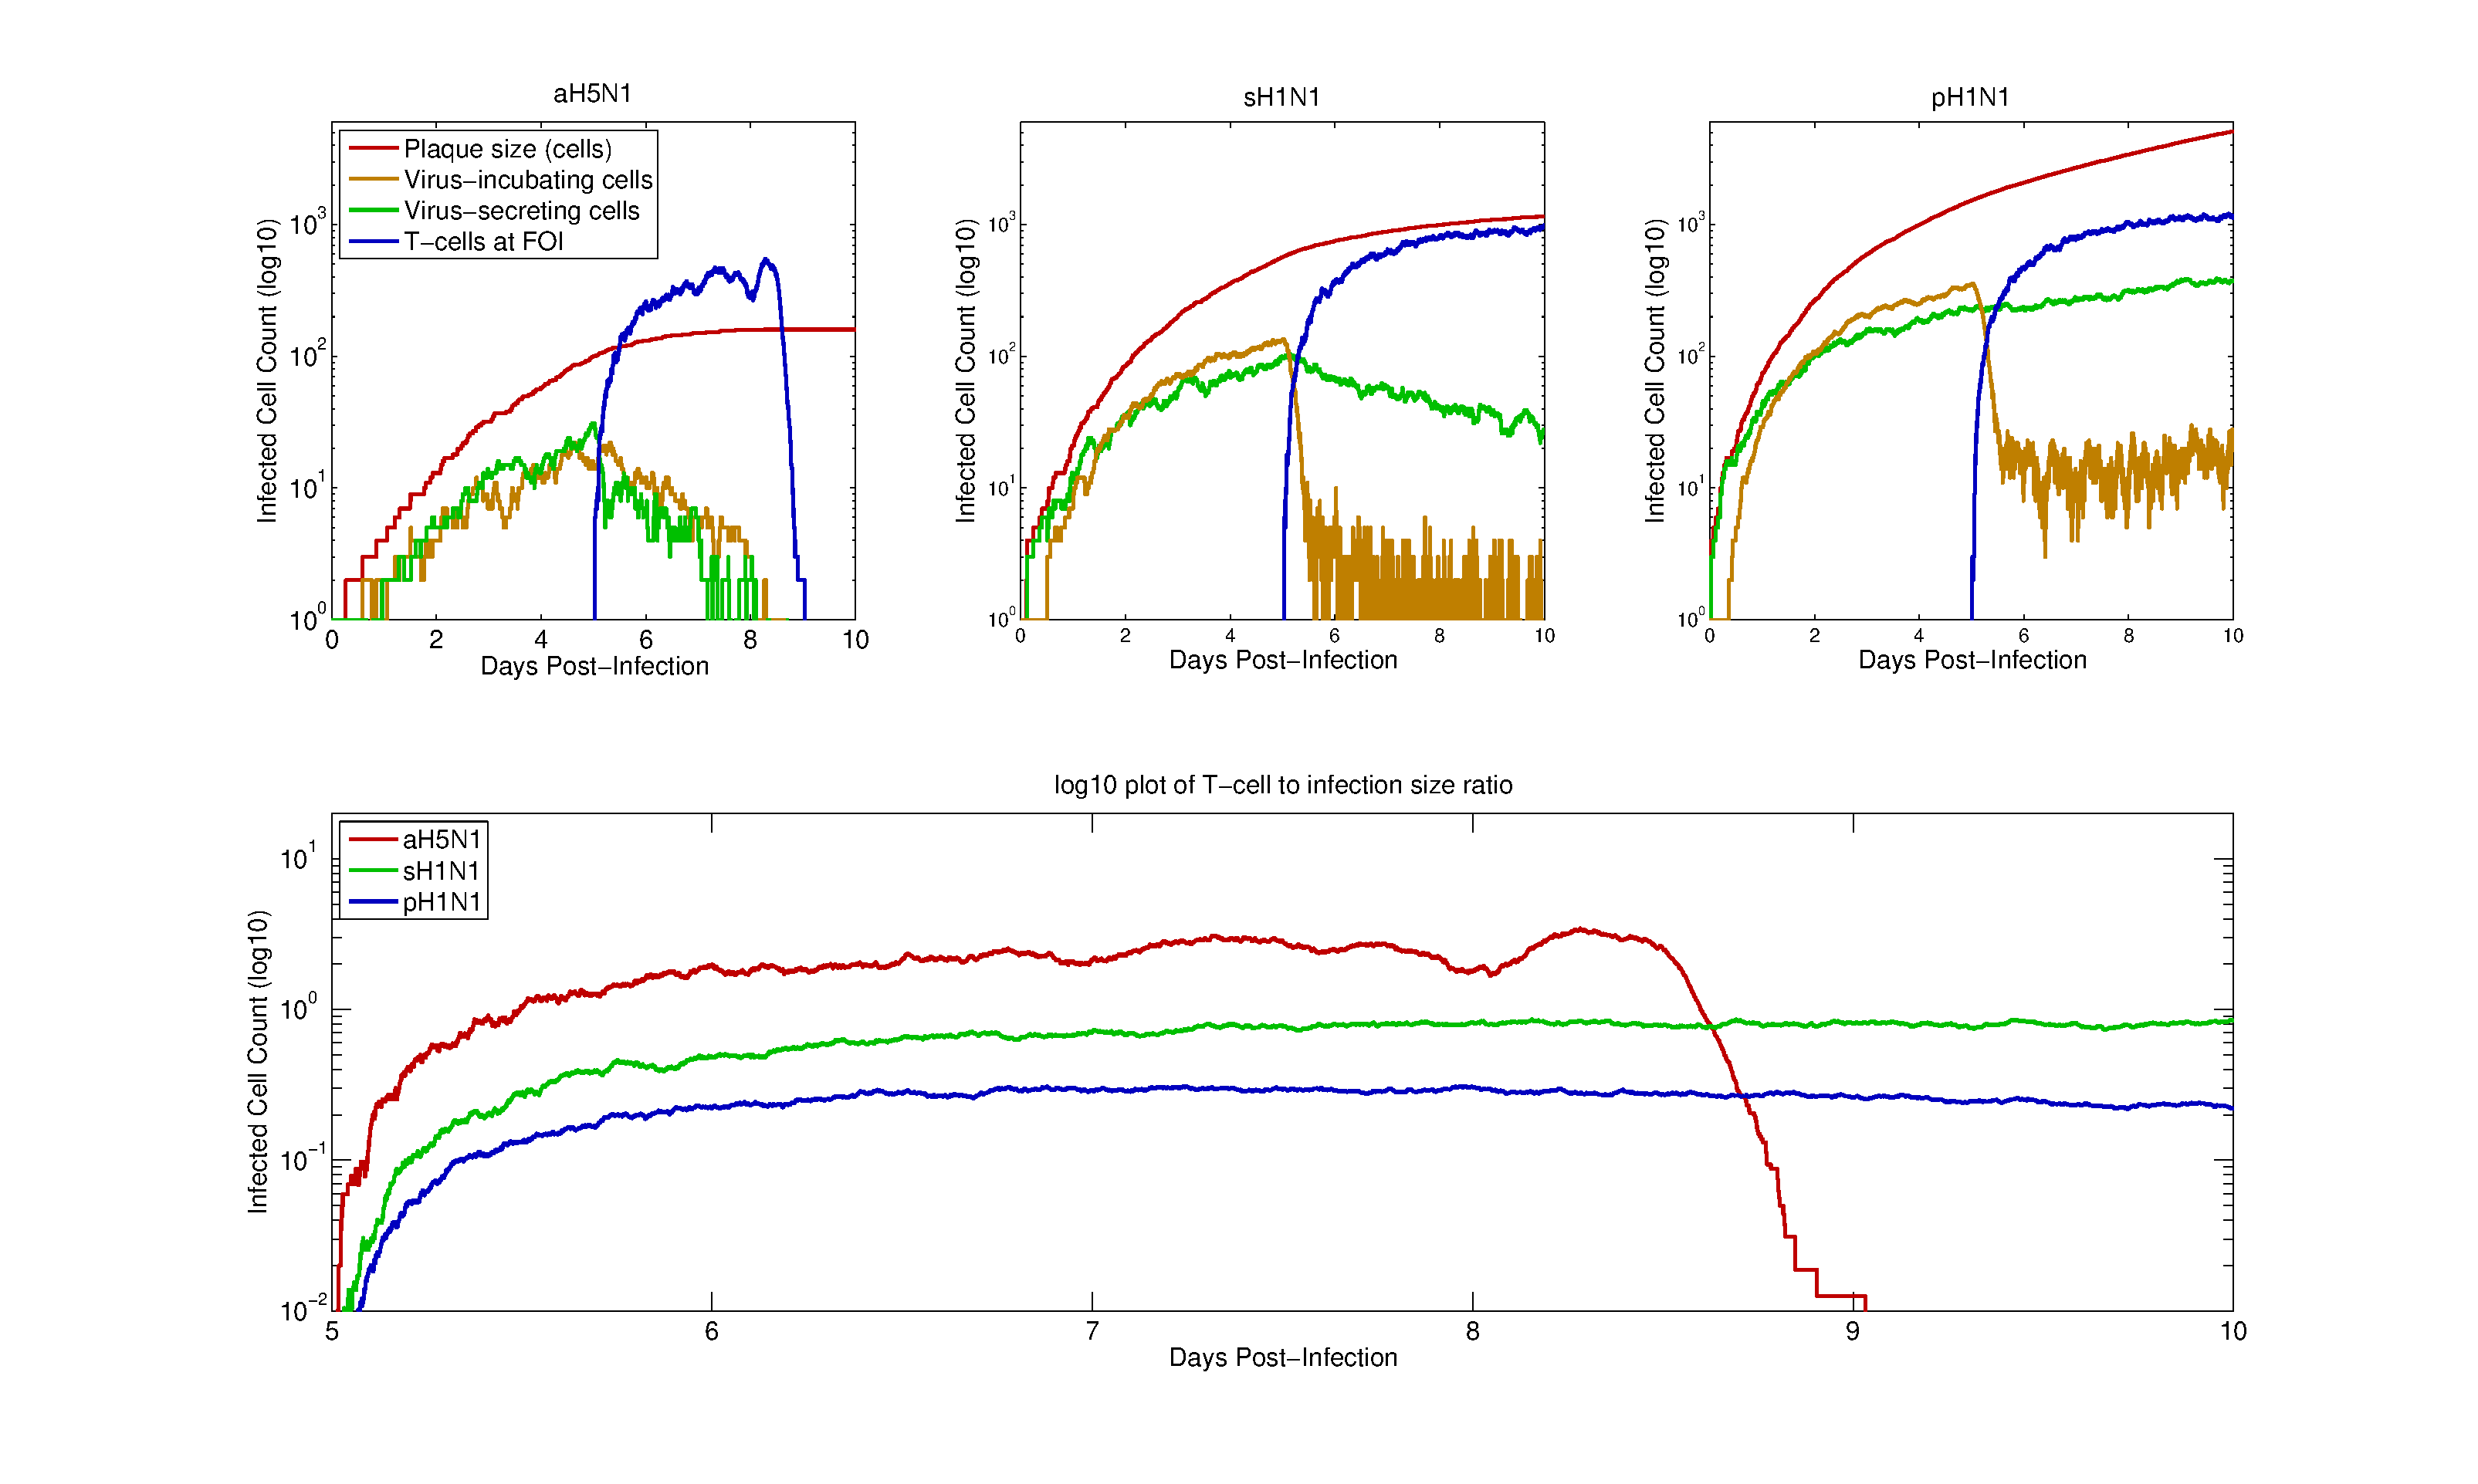
\includegraphics[width=0.7\textwidth]{tcellratio}
 \end{center}
\caption{A logarithmic plot of the ratio of T-Cells at the focus of infection vs the number of cells that make up the focus of infection.  aH5N1 exhibits unstable behavior once the infection is cleared and T-cell counts are reduced to negligible levels.} 
 \label{fig:tcellratio}
\end{figure}


\begin{figure}[ht!]
\begin{center}
 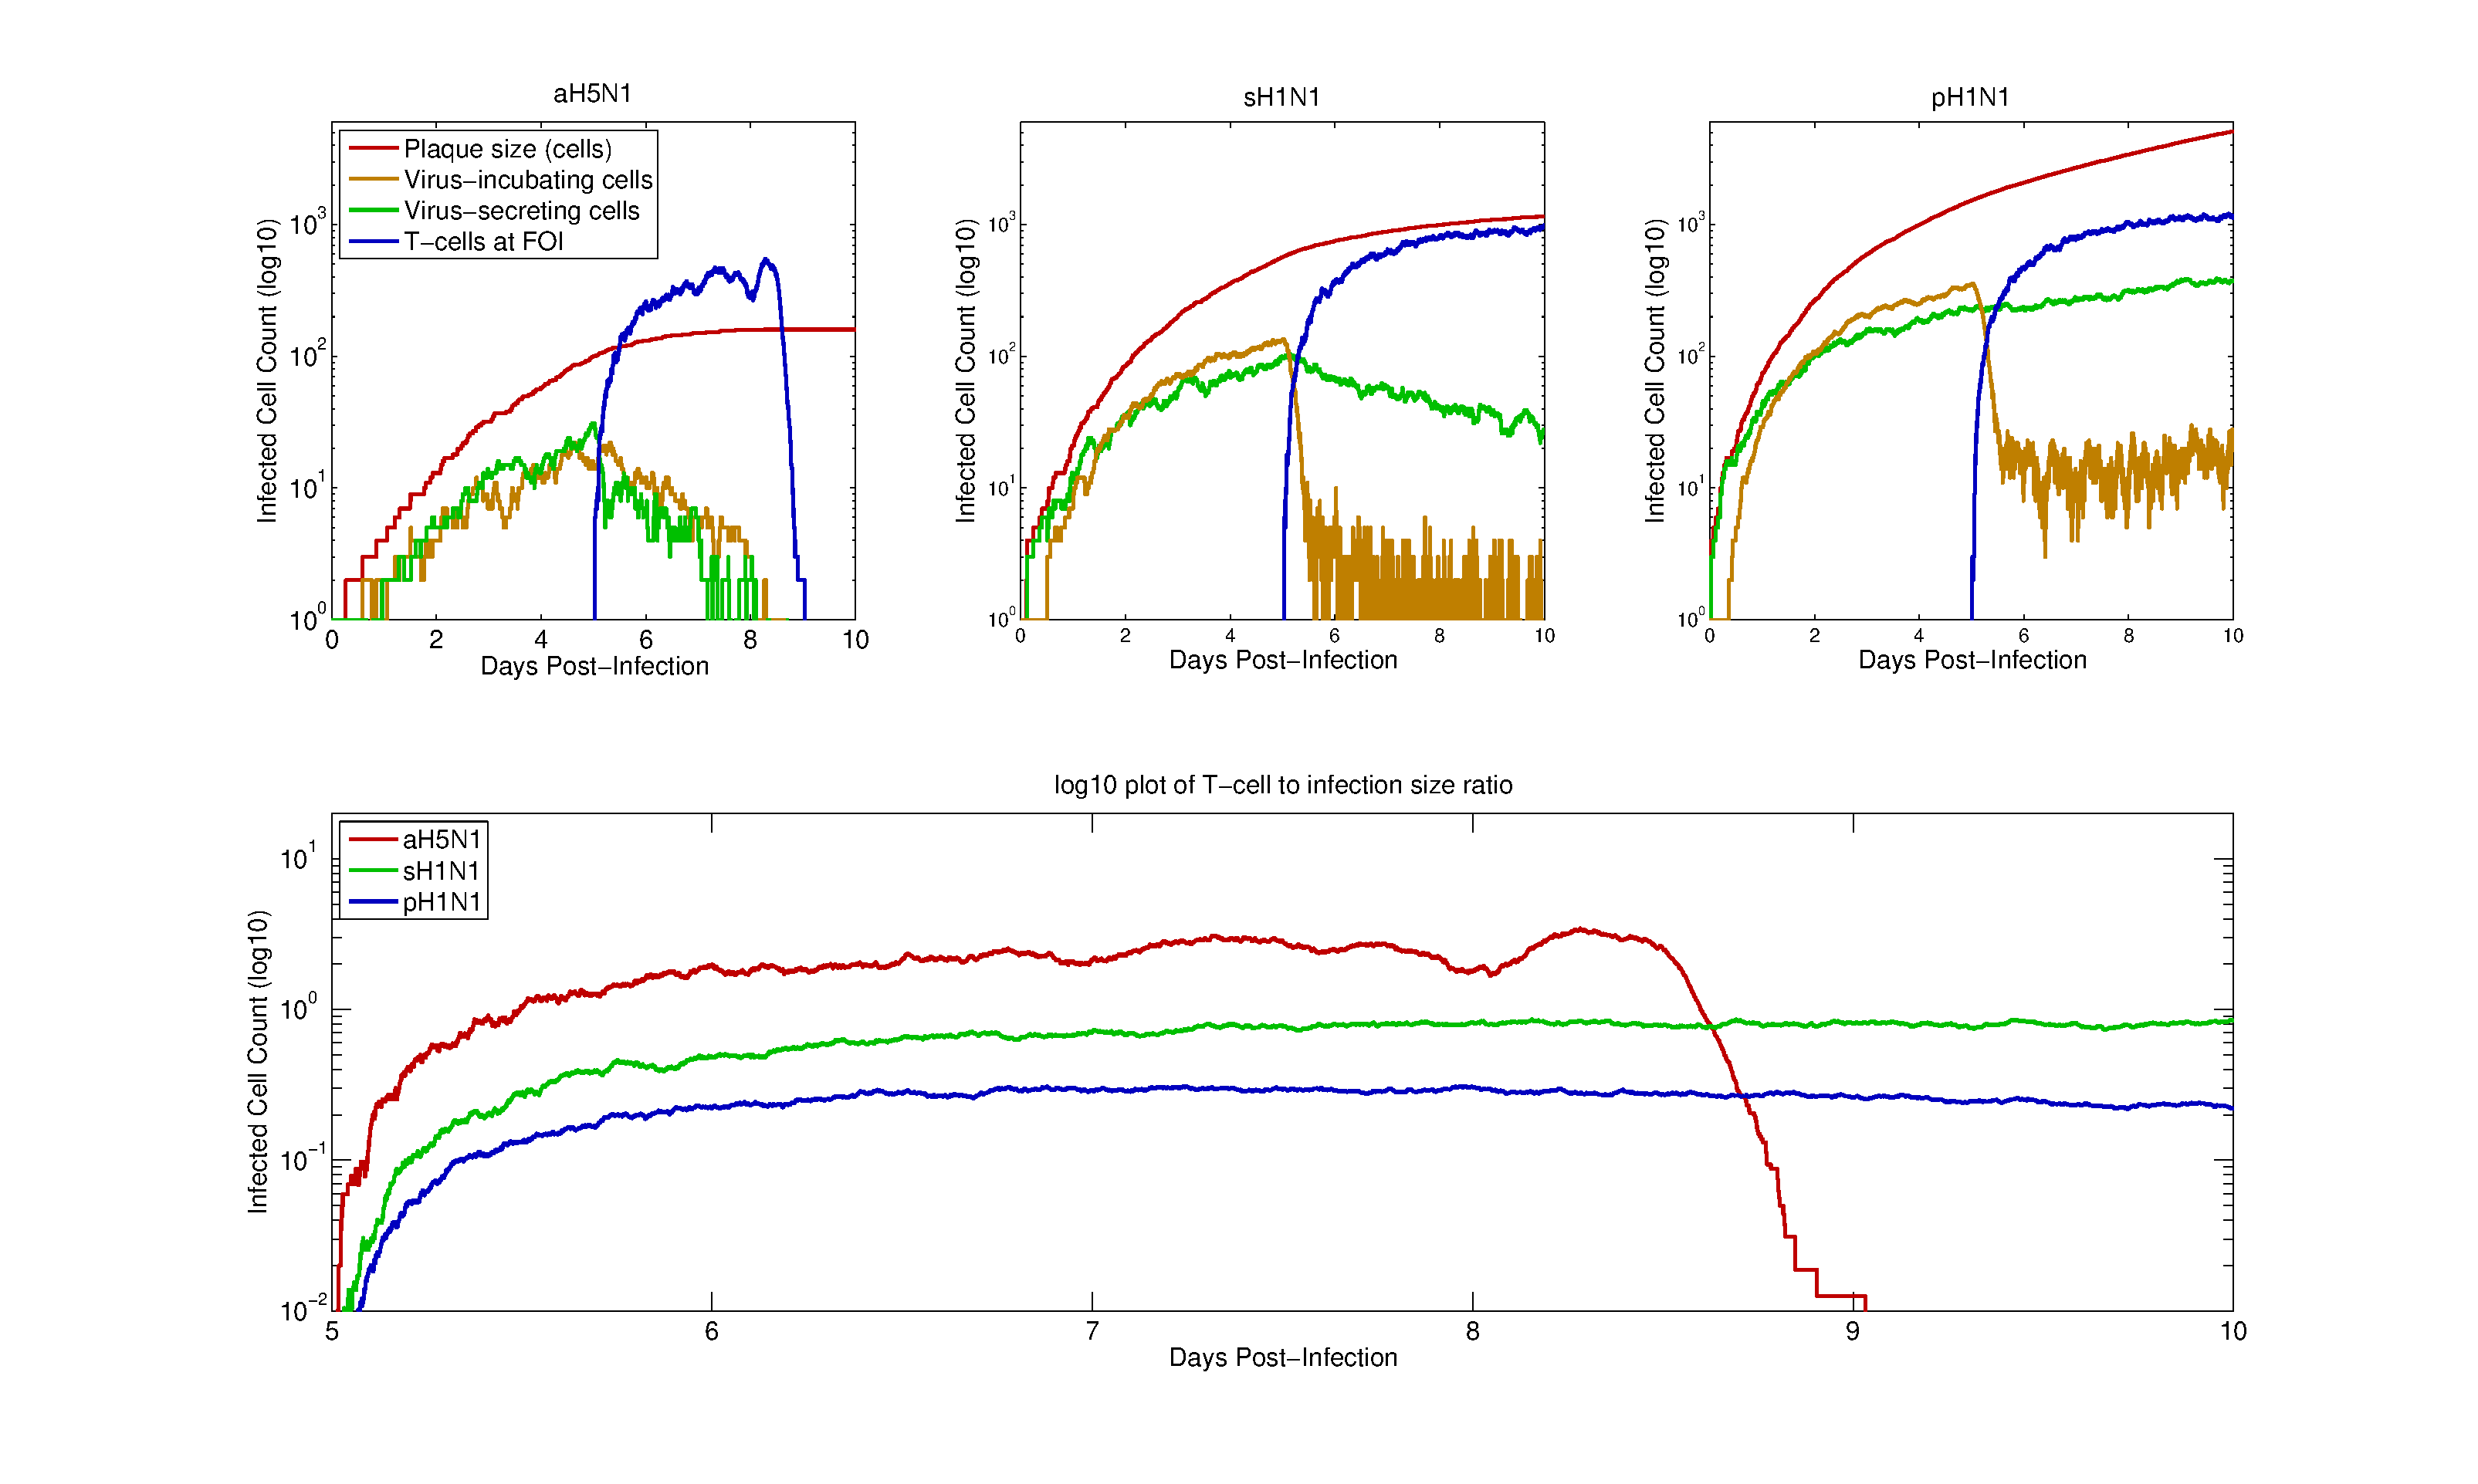
\includegraphics[width=\textwidth]{plaquesize}
 \end{center}
\caption{Comparison of total plaque size (green), number of virus incubating cells (blue), number of virus secreting cells (red), and T-cells (indigo) for the simulated infections of H5N1, sH1N1, and pH1N1.  NOTE TO SELF: Text came out tiny!  Legend is outdated.} 
 \label{fig:plaquesize}
\end{figure}


\section*{Discussion}

\subsection*{ABM Advantages}

The use of an ABM has advantages over a spatially homogeneous ODE model.  An ODE model assumes that any virus particle is capable of infecting any healthy cell.  Figure \ref{fig:cycells} shows that this is clearly not the case.  In fact, most free virus exists on top of infected cells that are no longer candidates for viral binding and fusion.  ODE models account for this discrepancy by lowering rates of infection by a constant amount, but this assumes that the proportion of unsuitable virions will always be the same.  This is clearly false as can been seen in Figure~\ref{fig:cycells} where the early infection has a higher proportion of virus overlapping healthy cells.

Another advantage of our ABM is the ability to render the model using OpenGL (Fig.~\ref{fig:cycells}).  The ability to see the model in action reveals spatial dynamics that are absent in ODE models and difficult or impossible to observe in \textit{in vitro} and \textit{in vivo} systems.  For example, observing the simulation reveals challenges to T-cell detection of infected cells that are not apparent using standard population plots.  By watching the model progress, we observed three key phenomena.  First, because T-cells find infected cells by climbing the chemokine gradient, we see T-cell clustering at local maxima of chemokine concentration.  Thus, we have an explanation for why T-cells do not increase in effectiveness as their numbers increase.  Second, we notice that clumps of T-cells remain in place even after all virus-secreting cells have been killed off.  This is because it takes time for the local chemokine maxima to diffuse and decay to a point where the T-cells can once again climb the gradient to a new maxima.  Finall, we can see that infected cells grow more disperse as the size of the infection grows.  Because T-cells cluster together they become incapable of covering the increasing plaque size.  These spatial observations provide explanations for the pH1N1 resurgence that would be hidden without the visualization tools provided by the ABM.


\subsection*{Model Comparison}

Hypercytokinemia is a characteristic of virulent influenza strains \cite{DeJong2006} but bloodstream levels of cytokines and chemokines may not reflect local concentrations and dynamics critical in guiding T cells to infected epithelial cells.  We elected to use our data on in vitro secretion of chemokines by human bronchial epithelial (NHBE) cells obtained from the same cultures of the three virus strains previously reported \cite{Mitchell2011}.  In this study the replication kinetics and productivity of the three virus strains were markedly different, but monolayer infection was initiated with a low MOI of 0.01 or 0.001, mimicking the initial infection naturally.  The levels of the chemokines CCL5 and CXCL10 in the basal media induced by the 3 strains were approximately equivalent at 24h post-infection.  When the productivity per cell was calculated, the avian H5N1 strain induced higher secretion of CCL5 (RANTES) than the seasonal or pandemic strains.  Greater CCL5 secretion by H5N1 strains has been noted in in vitro NHBE cultures when a relatively high MOI is used compared to seasonal strains \cite{Chan2005, Chan2010, Zeng2011} and pandemic strains \cite{Zeng2011}.  MOI and degree of differentiation of NHBE are critical determinants of cyto/chemokine secretion \cite{Chan2010}.  However, in spite of the attenuated type 1 interferon response induced by H5N1 strains \cite{Zeng2007}, the chemokine secretion is not attenuated.

Chemokines with a clear role directing T cell traffic include CXCL10 \cite{Dufour2002}, CCL5 \cite{Kawai1999} and CCL3 \cite{Kawai1999}.  The chemokine receptor CCR5, binding CCL5 and other chemokines, is crucial in the accelerated recruitment of CD8+ T cells to lung airways \cite{Kohlmeier2008}.  Other chemokines are likely to play a role in T cell traffic.  Although we did not detect significant levels of other chemokines in our cultures, the neutrophil- and T cell-attractant CXCL8/IL-8 is secreted into seasonal influenza-infected NHBE cultures \cite{Matsukura1996, Arndt2002}.  In the intact animal immigrant inflammatory cells particularly macrophages augment the multiple chemokine signals \cite{Julkunen2000}.  Finally, antigen-specific CD8+ T cell recognition of its target will induced lung injury mediated by TNFa and trigger addition alveolar epithelial cell chemokine secretion \cite{Zhao2000}.   Thus our model represents only a portion of the complete chemokine signal complex operating in the infected animal.

A key determinant in the efficiency of chemokine-directed T cell migration towards virus-secreting epithelial cells is the communication distance, defined by the threshold of sufficient chemokine signal to induce directed motion of the cell up the chemical gradient \cite{Thelen2008}.  The diameter of this cloud generated by a single cell is a function of production rate, decay rate, protein diffusion and the sensitivity threshold.  For the threshold of 100 pg/mL and maximal levels of concentration in tissue of 10,000 pg/mL, we calculated the effective communication distance as approximately 250 microns in our model.  This calculation matches the distance calculated for generic cytokines secreted by a suspended solitary cell \cite{Francis1997}.


\subsection*{Caveats and Limitations}

In both H1N1 strains the T-cell resposne fails to clear the infection by day 10.  In the case of pandemic H1N1, the infection continues to accelerate after a short period of clearance.  We suggest that this is due to the absence of several innate immune agents that were not included in the model.  We chose to remove most of the innate response in order to better focus on the relative effects of the cytokine signaling and T-cell response.  Although the infections do not clear by day 10, the models show clear differences in the ability of the immune system to deal with influenza strains of varying replication rates.  We see that the viral production rate is a major factor in the strength of the infection.

\subsection*{Future Work}



\section*{Materials}

Chemokine secretion:  Epithelial cell culture and supernatant collection was performed as described \cite{Mitchell2011}.  Briefly, undifferentiated human tracheal epithelial cells (University of Miami) were cultured for 4 weeks to achieve fully differentiated confluent monolayers on collagen-coated transwell inserts, or commercial differentiated human bronchial epithelial cells (EpiAirway Tissue, MatTek Corp., Ashland, MA) used immediately upon receipt, were infected at an MOI of 0.01 with either a seasonal H1N1 virus A/New Caledonia/20/99 (sH1N1), the 2009 H1N1 pandemic strain A/California/04/09 (pH1N1), or an avian H5N1 virus A/Hong Kong/483/97 (aH5N1) derived from a fatal human infection.  Apical fluid for viral secretion, and basal media for chemokine secretion collected before treatment of the monolayer with protease, was collected from previously undisturbed triplicate or quadruplicate wells at 0, 6, 10, 12, 16, 20, 24, 30, 36, 42, 48, and 72 hours after infection, and stored at -80C until assay.  Quantitative viral culture was performed by standard plaque assay.  Quantitative chemokine levels were performed in 30 µl aliquots for a panel of 17 chemokines and cytokines (Luminex Assay®, Luminex Corp.) and reported as ng/mL basal media sampled from a total volume of 4 mL.

% Do NOT remove this, even if you are not including acknowledgments
\section*{Acknowledgments}


\section*{References}
% The bibtex filename
\bibliography{references}

\section*{Figure Legends}
%\begin{figure}[!ht]
%\begin{center}
%%\includegraphics[width=4in]{figure_name.2.eps}
%\end{center}
%\caption{
%{\bf Bold the first sentence.}  Rest of figure 2  caption.  Caption 
%should be left justified, as specified by the options to the caption 
%package.
%}
%\label{Figure_label}
%\end{figure}


\section*{Tables}
%\begin{table}[!ht]
%\caption{
%\bf{Table title}}
%\begin{tabular}{|c|c|c|}
%table information
%\end{tabular}
%\begin{flushleft}Table caption
%\end{flushleft}
%\label{tab:label}
% \end{table}

\end{document}

